\section{Introduction}

\plainMHCI{} molecules display intracellularly derived peptides at the cell surface for surveillance by cytotoxic CD8\(^{+}\) T cells. The resulting immunopeptidome is shaped by substantially more than peptide binding to an \plainMHC{}: protein abundance and turnover, proteolytic degradation, antigen-processing pathways, cellular composition, tissue environment, and experimental detectability can all affect which peptides are observed. Multi-tissue immunopeptidomic studies have consequently revealed both widely shared ligands and pronounced tissue-associated differences \cite{marcu2021atlas,schuster2018mouse}. Nevertheless, most computational models are designed to predict peptide binding to or presentation by an \plainMHC{} in a general setting and therefore do not directly characterize how presentation evidence varies across tissues under a fixed MHC context.

Tissue-associated presentation preference by \plainMHCI{} can arise at several successive stages of antigen processing. Genes encoding constitutive or immunoproteasomal subunits, TAP1/2 transporters, ERAP1/2 aminopeptidases, and components of the peptide-loading machinery are not expressed uniformly across tissues. Together with tissue-dependent source-protein abundance and cell-type composition, these differences can alter which proteins are cleaved, which peptide fragments enter the endoplasmic reticulum, how precursor peptides are trimmed, and which sufficiently stable peptide--\plainMHCI{} complexes are ultimately displayed at the cell surface \cite{kubiniok2022constitutive}. Thus, the same source protein may generate different presented epitopes in different tissues, while the same epitope may differ across tissues in the amount or likelihood of surface presentation. Understanding this variation is important for cancer therapy: it can help prioritize epitopes that are efficiently presented by tumors but minimally presented by essential normal tissues, thereby improving target selection and reducing potential on-target, off-tumor toxicity. In the present study, these mechanisms provide a biological explanation for tissue-associated preference rather than a causal claim, because the model does not directly measure gene expression or the activity of individual processing steps.

Figure~\ref{fig:tissue-specific-presentation-mechanism} summarizes these mechanisms and the biological motivation for tissue-conditioned presentation.

\begin{figure*}[t]
\centering
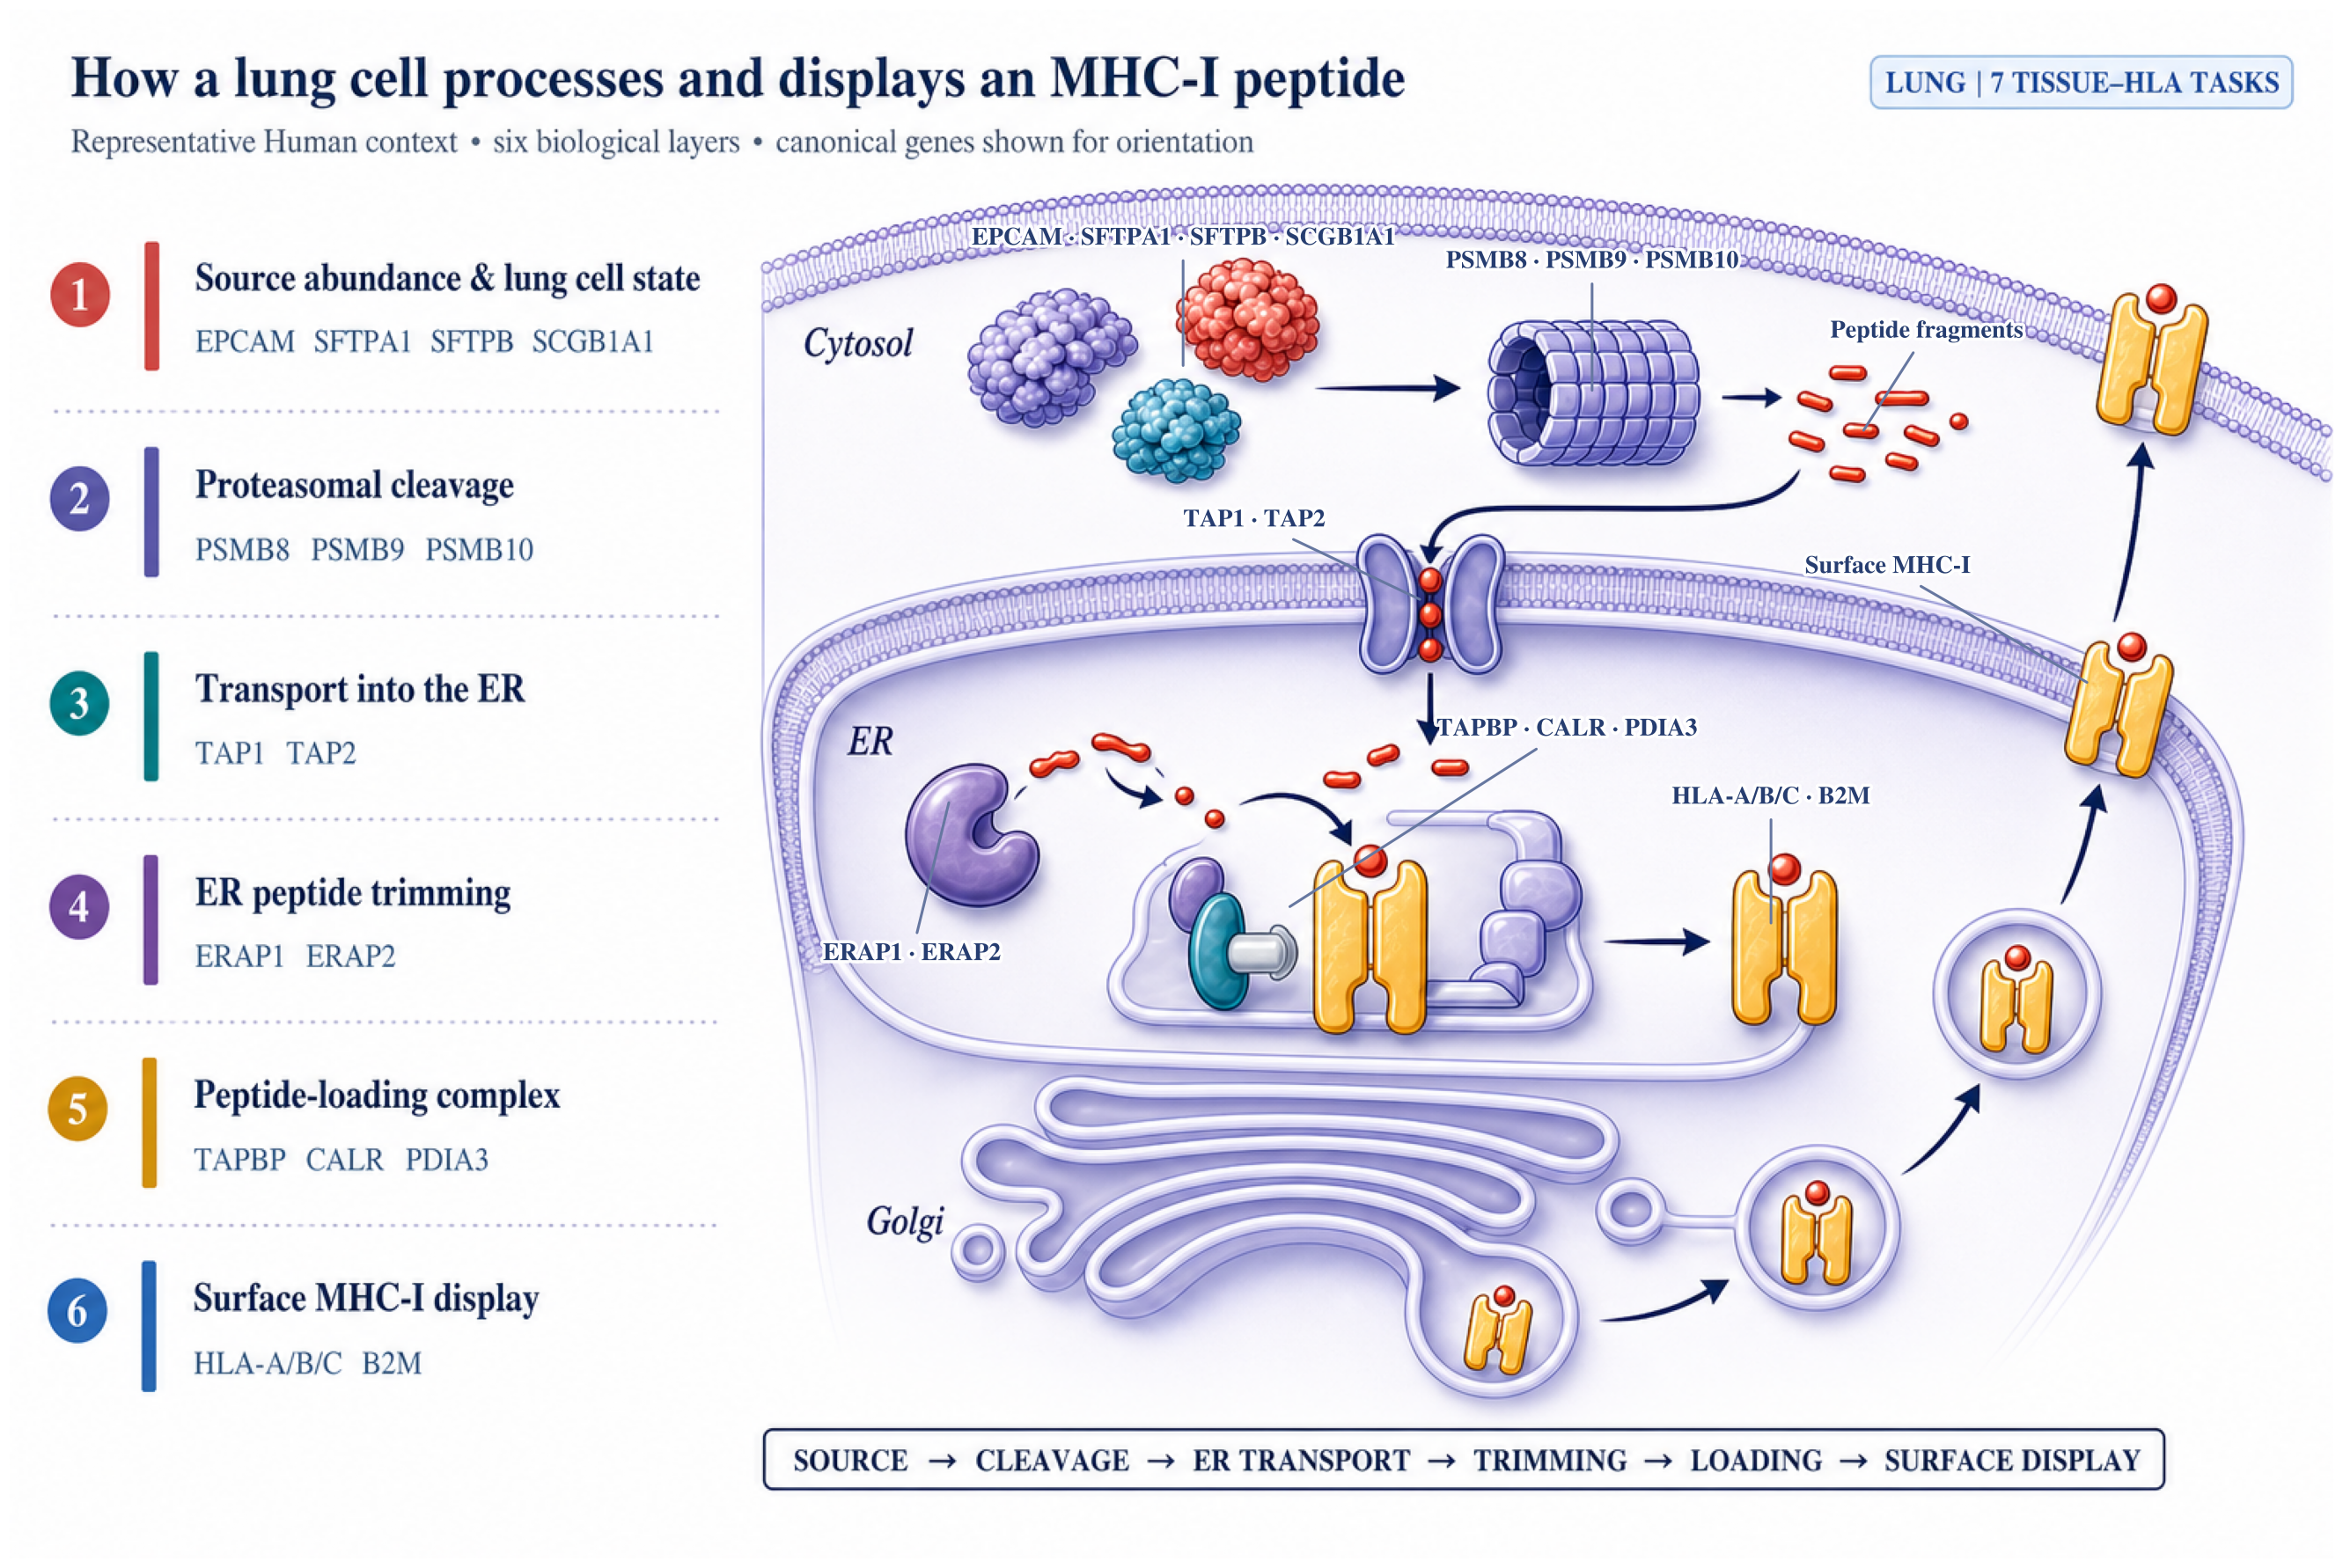
\includegraphics[width=\textwidth]{figures/figure1_lung_presentation_pathway_v3.png}
\caption{Representative antigen-processing pathway in a Human lung epithelial context. Lung is shown because it contributes seven retained tissue--HLA tasks, providing a multi-allele example without implying that the depicted pathway is lung-exclusive. Tissue and cell state affect source-protein abundance (illustrative lung markers: \emph{EPCAM}, \emph{SFTPA1}, \emph{SFTPB}, and \emph{SCGB1A1}); immunoproteasome components such as \emph{PSMB8--10} cleave cytosolic proteins; \emph{TAP1/2} transport fragments into the endoplasmic reticulum; \emph{ERAP1/2} trim precursors; the loading complex, including \emph{TAPBP}, \emph{CALR}, and \emph{PDIA3}, supports peptide loading; and \plainHLA{}-A/B/C with \emph{B2M} forms the surface \plainMHCI{} complex. The gene labels identify canonical biological components for orientation; they are not direct model inputs or causal measurements in this study.}
\label{fig:tissue-specific-presentation-mechanism}
\end{figure*}

Existing tools answer related but different questions. Some estimate whether a peptide can bind an \plainMHC{}; others estimate whether it is likely to be presented in a pooled or sample-specific setting, sometimes using expression or processing information \cite{reynisson2020netmhcpan,odonnell2020mhcflurry,albert2023bigmhc}. Here we ask a narrower relative question: when the MHC allele and source protein are held constant, which of two peptides has stronger evidence in one specified tissue? Holding these two factors constant reduces easy explanations based only on peptide--MHC compatibility or protein identity and makes tissue-associated differences the focus of the comparison.

We call this question tissue--MHC-specific presentation preference prediction. Each prediction context corresponds to one tissue and one MHC restriction. Let \(p\) denote a peptide and let \(\tau=(t,m)\) denote that tissue--MHC combination. A model produces a score
\[
s_{\theta}(p,\tau)\in\mathbb{R},
\]
which is used to rank peptides within that combination. A larger score means stronger predicted evidence relative to other candidates in the same context; it is not an absolute probability that the peptide is present. The model is evaluated only for tissue--MHC combinations represented during training, so it should not be interpreted as a predictor for a new tissue, a new MHC allele, or a new tissue--MHC combination.

To construct training examples aligned with this objective, each recorded-positive peptide is paired with a comparison peptide that has evidence elsewhere but not in the target tissue (a pseudo-negative peptide) under the constraints
\[
m^{+}=m^{-}, \qquad u^{+}=u^{-},
\]
where \(m\) is the MHC restriction and \(u\) is the parent UniProt protein. One peptide is reported in the target tissue; its comparison peptide is reported elsewhere under the same MHC and from the same protein, but not in the target context. Biologically, the pair asks whether two fragments of one protein show different tissue-associated evidence after controlling the presenting allele and source-protein identity. The second peptide is a pseudo-negative rather than a confirmed biological absence. Missing reports can reflect incomplete sampling or limited mass-spectrometry detection, and the pairing cannot remove study, batch, expression, or cell-composition effects.

On this basis, we introduce paired human and mouse TissuePMHC benchmarks and separately trained species-specific prediction models. Each model combines a globally shared peptide representation with a representation restricted to one MHC allele; in biological terms, this allows broadly shared sequence patterns and allele-associated motifs to contribute separately. To prevent total cross-tissue reporting frequency from separating the labels, the two members of every pair have the same number of positive tissue occurrences. Evaluation uses one fixed internal train/test split per species, with 50 test pairs per retained tissue--MHC combination and three independent final-training seeds. Species-specific hyperparameters are selected by cross-validation confined to the training split before the fixed test is opened. A held-out peptide is absent from fitting rows for the same combination but may recur in another combination.

The study makes five main contributions. First, it defines a biologically motivated comparison in which MHC restriction, parent protein, and total positive tissue-occurrence count are matched. Second, it provides Human and Mouse benchmarks with the same fixed-test allocation of 50 pairs per retained tissue--MHC combination. Third, it verifies pairwise and taskwise that occurrence-count distributions are identical between labels, making this count alone exactly non-discriminative. Fourth, it tests whether the retained signal depends on tissue identity or can be explained by general peptide--MHC compatibility alone. Fifth, it combines task-conditional branch-level attribution with exhaustive single-residue perturbation to identify and independently validate peptide positions and HLA-stratified residue patterns used by the Human model, and then tests whether a fixed substitution has different fitted effects across tissues sharing the same HLA. The aim is therefore not only to report a score, but also to state which shortcut has been controlled, what sequence evidence the model uses, and which observational limitations remain. After the background, the paper proceeds from data and task definition to balance and leakage audits, the model and evaluation protocol, primary Human and Mouse results, strict-generalization scope, component and interpretation analyses, tissue and allele heterogeneity, and finally external controls.
